\documentclass[large,ignorenonframetext,aspectratio=169,]{paradise-slide}
\setbeamertemplate{caption}[numbered]
\setbeamertemplate{caption label separator}{:}
\setbeamercolor{caption name}{fg=normal text.fg}
\usepackage{amssymb,amsmath}
\usepackage{ifxetex,ifluatex}
\usepackage{fixltx2e} % provides \textsubscript

% use upquote if available, for straight quotes in verbatim environments
\IfFileExists{upquote.sty}{\usepackage{upquote}}{}
% use microtype if available
\IfFileExists{microtype.sty}{\usepackage{microtype}}{}
\usepackage{url}
\usepackage{graphicx}
\makeatletter
\def\maxwidth{\ifdim\Gin@nat@width>\linewidth\linewidth\else\Gin@nat@width\fi}
\def\maxheight{\ifdim\Gin@nat@height>\textheight0.8\textheight\else\Gin@nat@height\fi}
\makeatother
% Scale images if necessary, so that they will not overflow the page
% margins by default, and it is still possible to overwrite the defaults
% using explicit options in \includegraphics[width, height, ...]{}
\setkeys{Gin}{width=\maxwidth,height=\maxheight,keepaspectratio}

% Comment these out if you don't want a slide with just the
% part/section/subsection/subsubsection title:
\AtBeginPart{
  \let\insertpartnumber\relax
  \let\partname\relax
  \frame{\partpage}
}
\AtBeginSection{
  \let\insertsectionnumber\relax
  \let\sectionname\relax
  \frame{\sectionpage}
}
\AtBeginSubsection{
  \let\insertsubsectionnumber\relax
  \let\subsectionname\relax
  \frame{\subsectionpage}
}

\setlength{\parindent}{0pt}
\setlength{\emergencystretch}{3em}  % prevent overfull lines
\providecommand{\tightlist}{%
  \setlength{\itemsep}{0pt}\setlength{\parskip}{0pt}}
\setcounter{secnumdepth}{0}
\usepackage{divine}
\usepackage{multirow}
\usepackage{tikz}
\usepackage{graphicx}
\usepackage{pbox}
\usepackage{booktabs}
\usepackage{siunitx}
\usetikzlibrary{shapes, arrows, shadows, positioning, calc, fit, backgrounds, decorations.pathmorphing}
\usetikzlibrary{trees}
\setbeamertemplate{caption}{\raggedright\insertcaption\par}
\newcommand{\columnsbegin}{\begin{columns}}
\newcommand{\columnsend}{\end{columns}}
\newcommand{\centerbegin}{\begin{center}}
\newcommand{\centerend}{\end{center}}

\title[DiOS]{Rozšíření DiOSu, interního operačního systému verifikačního nástroje
DIVINE}
\author{Petr Ročkai \and Jan Mrázek \and Zuzana Baranová}
\date{26. listopadu 2018}

\begin{document}
\frame[plain]{\titlepage}

\begin{frame}{DIVINE 4}
\protect\hypertarget{divine-4}{}

\begin{itemize}
\tightlist
\item
  explicitní model-checker pro C/C++
\item
  vyvíjen v laboratoři ParaDiSe
\item
  cílí na verifikaci paralelního a reálného kódu
\end{itemize}

\centering
\bigskip

\url{https://divine.fi.muni.cz}

\end{frame}

\begin{frame}{Architektura DIVINE 4}
\protect\hypertarget{architektura-divine-4}{}

\begin{figure}
\centering
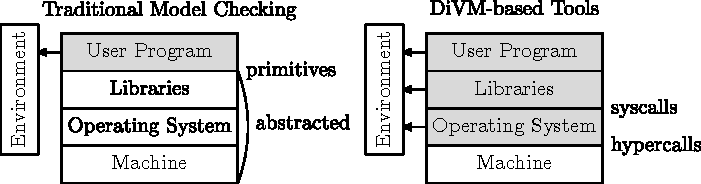
\includegraphics{divine_arch.pdf}
\caption{Klasický model-checker vs.~DIVINE 4}
\end{figure}

\end{frame}

\begin{frame}{DiOS}
\protect\hypertarget{dios}{}

\begin{itemize}
\tightlist
\item
  ``modelový'' operační systém

  \begin{itemize}
  \tightlist
  \item
    není bootovatelný
  \item
    běží nad rozhraním DiVM
  \item
    simuluje vstupně-výstupní operace
  \end{itemize}
\item
  POSIXové rozhraní

  \begin{itemize}
  \tightlist
  \item
    libc \& libstdc++
  \item
    pthread
  \item
    filesystem
  \end{itemize}
\end{itemize}

\end{frame}

\begin{frame}{Cíl projektu}
\protect\hypertarget{cuxedl-projektu}{}

Rozšířit DiOS a k němu příslušné nástroje.

\begin{itemize}
\tightlist
\item
  modularizace a konfigurovatelnost systému
\item
  implementace podpory pro procesy
\item
  implementace podpory pro synchronní systémy
\item
  implementace fairness pro scheduler
\item
  integrace DiOSu s DIVINE simulátorem
\end{itemize}

\end{frame}

\begin{frame}{Modularizace, konfigurovatelnost, schedulery}
\protect\hypertarget{modularizace-konfigurovatelnost-schedulery}{}

\begin{itemize}
\tightlist
\item
  DiOS rozdělen na téměř nezávislé komponenty

  \begin{itemize}
  \tightlist
  \item
    scheduler, process manager, fault handler, virtual file system,
    \ldots{}
  \item
    lze vypustit nepotřebné komponenty (např. procesy)
  \item
    lze vyměnit komponenty za specializované (fair nebo synchronní
    scheduler)
  \end{itemize}
\item
  konfigurace skrze vrstvení šablon
\end{itemize}

\pause

\begin{itemize}
\tightlist
\item
  konfigurovatelností nebyl zaznamenán žádný propad výkonu
\end{itemize}

\pause

\begin{itemize}
\tightlist
\item
  implementován fair scheduler (verifikace vlastností LTL)
\item
  implementován synchronní scheduler (verifikace Simulinkových diagramů)
\end{itemize}

\end{frame}

\begin{frame}[fragile]{Implementace podpory pro procesy}
\protect\hypertarget{implementace-podpory-pro-procesy}{}

\begin{itemize}
\tightlist
\item
  DiOS umí imitovat chování programů na bázi POSIXu
\item
  přibyla nová systémová komponenta
\end{itemize}

\pause

\begin{itemize}
\tightlist
\item
  výzvy během implementace:

  \begin{itemize}
  \tightlist
  \item
    ochrana paměti při forku
  \item
    implementace \texttt{kill} (volání na sebe sama a zajištění volání
    uživatelských handlerů)
  \end{itemize}
\end{itemize}

\end{frame}

\begin{frame}{Integrace DiOSu se simulátorem}
\protect\hypertarget{integrace-diosu-se-simuluxe1torem}{}

DIVINE simulátor byl vylepšen o:

\begin{itemize}
\tightlist
\item
  demanglování jmen funkcí
\item
  skrytí implementace DiOSu v simulátoru:

  \begin{itemize}
  \tightlist
  \item
    DiOS byl pro simulátor nerozeznatelný od uživatelského kódu
  \item
    výpisy zahlcovaly uživatele
  \item
    zavedeny jmenné aliasy, skákání po funkčních rámcích
  \end{itemize}
\item
  implementovány lepivé příkazy

  \begin{itemize}
  \tightlist
  \item
    užitečné např. pro vypsání útržku kódu, rámce apod.
  \item
    připodobňuje práci se simulátorem práci s GDB
  \end{itemize}
\item
  uživatelský manuál byl rozšířen o sekci práce s DiOSem a simulátorem
\end{itemize}

\end{frame}

\begin{frame}[fragile]{Závěr}
\protect\hypertarget{zuxe1vux11br}{}

\begin{itemize}
\tightlist
\item
  v rámci projektu jsme úspěšně:

  \begin{itemize}
  \tightlist
  \item
    udělali DiOS konfigurovatelným
  \item
    implementovali fair scheduler
  \item
    přidali do DiOSu podporu pro synchronní systémy
  \item
    přidali podporu pro POSIXové procesy
  \item
    zpříjemnili uživatelský zážitek
  \end{itemize}
\item
  nad rámec projektu jsme:

  \begin{itemize}
  \tightlist
  \item
    téměř zdvojnásobili sadu regresních testů pro DIVINE 4 (na 1200)
  \end{itemize}
\item
  výstupy začleněny do hlavní vývojové větve DIVINE
\end{itemize}

Projekt k nalezení na \texttt{https://divine.fi.muni.cz}.

\end{frame}

\end{document}
